\begin{savequote}
The retinal image produced by the hand of a gesticulating
speaker is never the same from moment to moment, yet the brain must consistently categorize
it as a hand. 
\qauthor{Semir Zeki, \textit{The visual image in mind and brain}}
\end{savequote}
\chapter{Hand Tracking}

\section{Kinect Sensor}
The depth sensor data from the Kinect is quite noisy. For a static scene, the
average absolute pixel difference from the RGB camera is about 0.6\% of the maximum value (8
bits), while the average absolute depth difference per pixel is about 4.2\%
(347.89mm) of the maximum value (13 bits).

The random error of depth measurements increases quadratically with increasing distance from the 
sensor and ranges from a few millimeters at 0.5m distance to about 4cm
at the maximum range of 5 meters \cite{khoshelham2011}.

With default range, the depth sensor has a normal range limit of about 0.8m -
4m.

\begin{figure}[tbh]
\centering
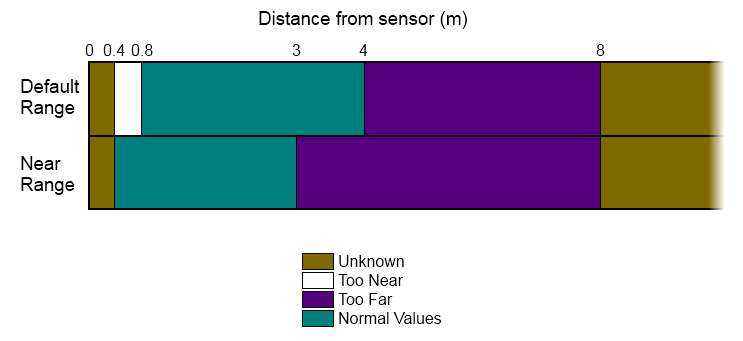
\includegraphics[width=\textwidth]{figures/kinect_sensor_range.png}
\caption{Kinect depth sensor range \cite{microsoft-kinect}.}
\end{figure}

\begin{figure}[tbh]
\centering
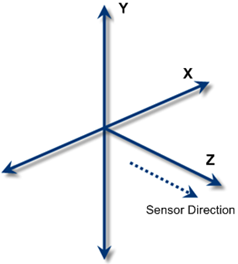
\includegraphics[width=0.3\textwidth]{figures/skeleton_space.png}
\caption{Kinect skeleton
space\footnote{http://msdn.microsoft.com/en-us/library/hh973078.aspx}}
\label{}
\end{figure}

\section{Wearable Sensors}
Each IMU provides linear acceleration, angular acceleration, magnetometer, Euler
orientation and orientation quaternion. The skeleton data from Kinect is prone
to occlusion and the quality of accuracy highly dependent on the position of the
user relatively to the sensor; IMU sensors are occlusion free and position
independent. While Kinect often requires complex processing to extract features
from video streams, data from IMUs can be used with less complex processing
\cite{Ruffieux2013}.

\section{Hand Tracking for Tabletop}
\subsection{System Setup}
The custom tabletop structure includes four $1280\times1024$ pixel projectors 
(Dell 5100MP) that provide a $2560\times2048$ pixel resolution display. The
display is projected onto a flat white surface digitizer (GTCO Calcomp DrawingBoard V), 
which uses a stylus as an input device. The digitizer is tilted 10 degrees down 
in front, and is placed at 41in (104cm) above the floor, following FAA's design 
standard to accommodate the $5^{th}$ through $95^{th}$ percentiles of 
population. The projected displays were mechanically aligned to produce a single 
seamless large display area. The graphics card used is AMD
Radeon\texttrademark{TM} HD 6870 and the operating system used is Ubuntu 11.10.

\begin{figure}
  \centering
  \subfigure[] {
	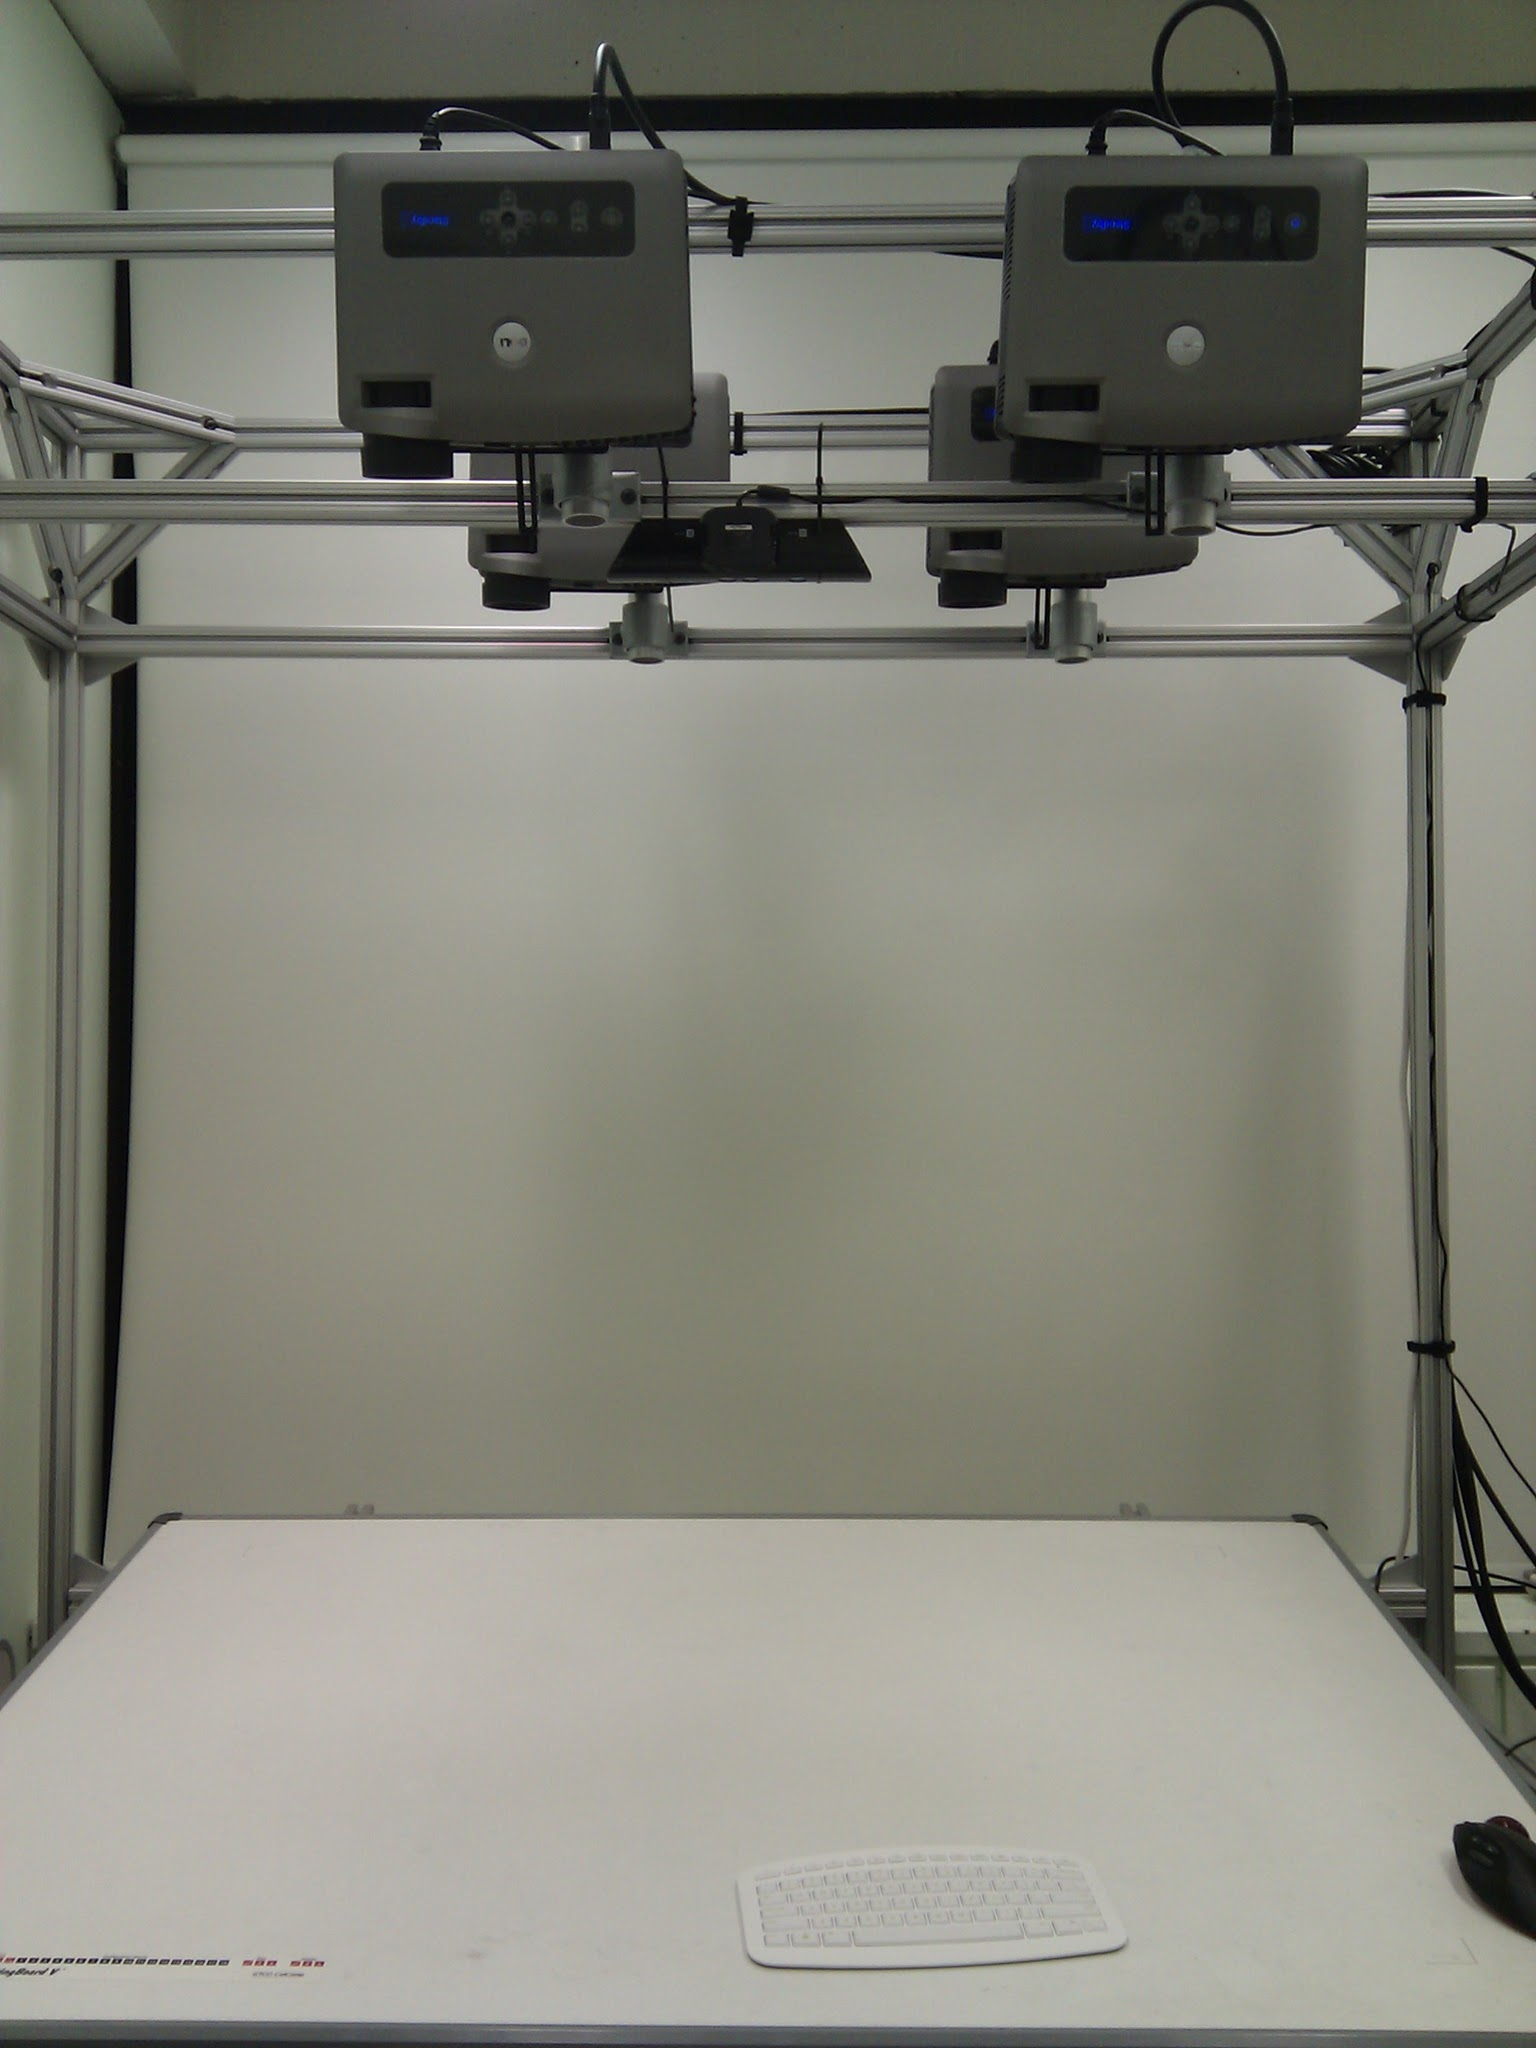
\includegraphics[width=0.4\textwidth]{figures/setup1.png} 
  }
  \subfigure[] {
  	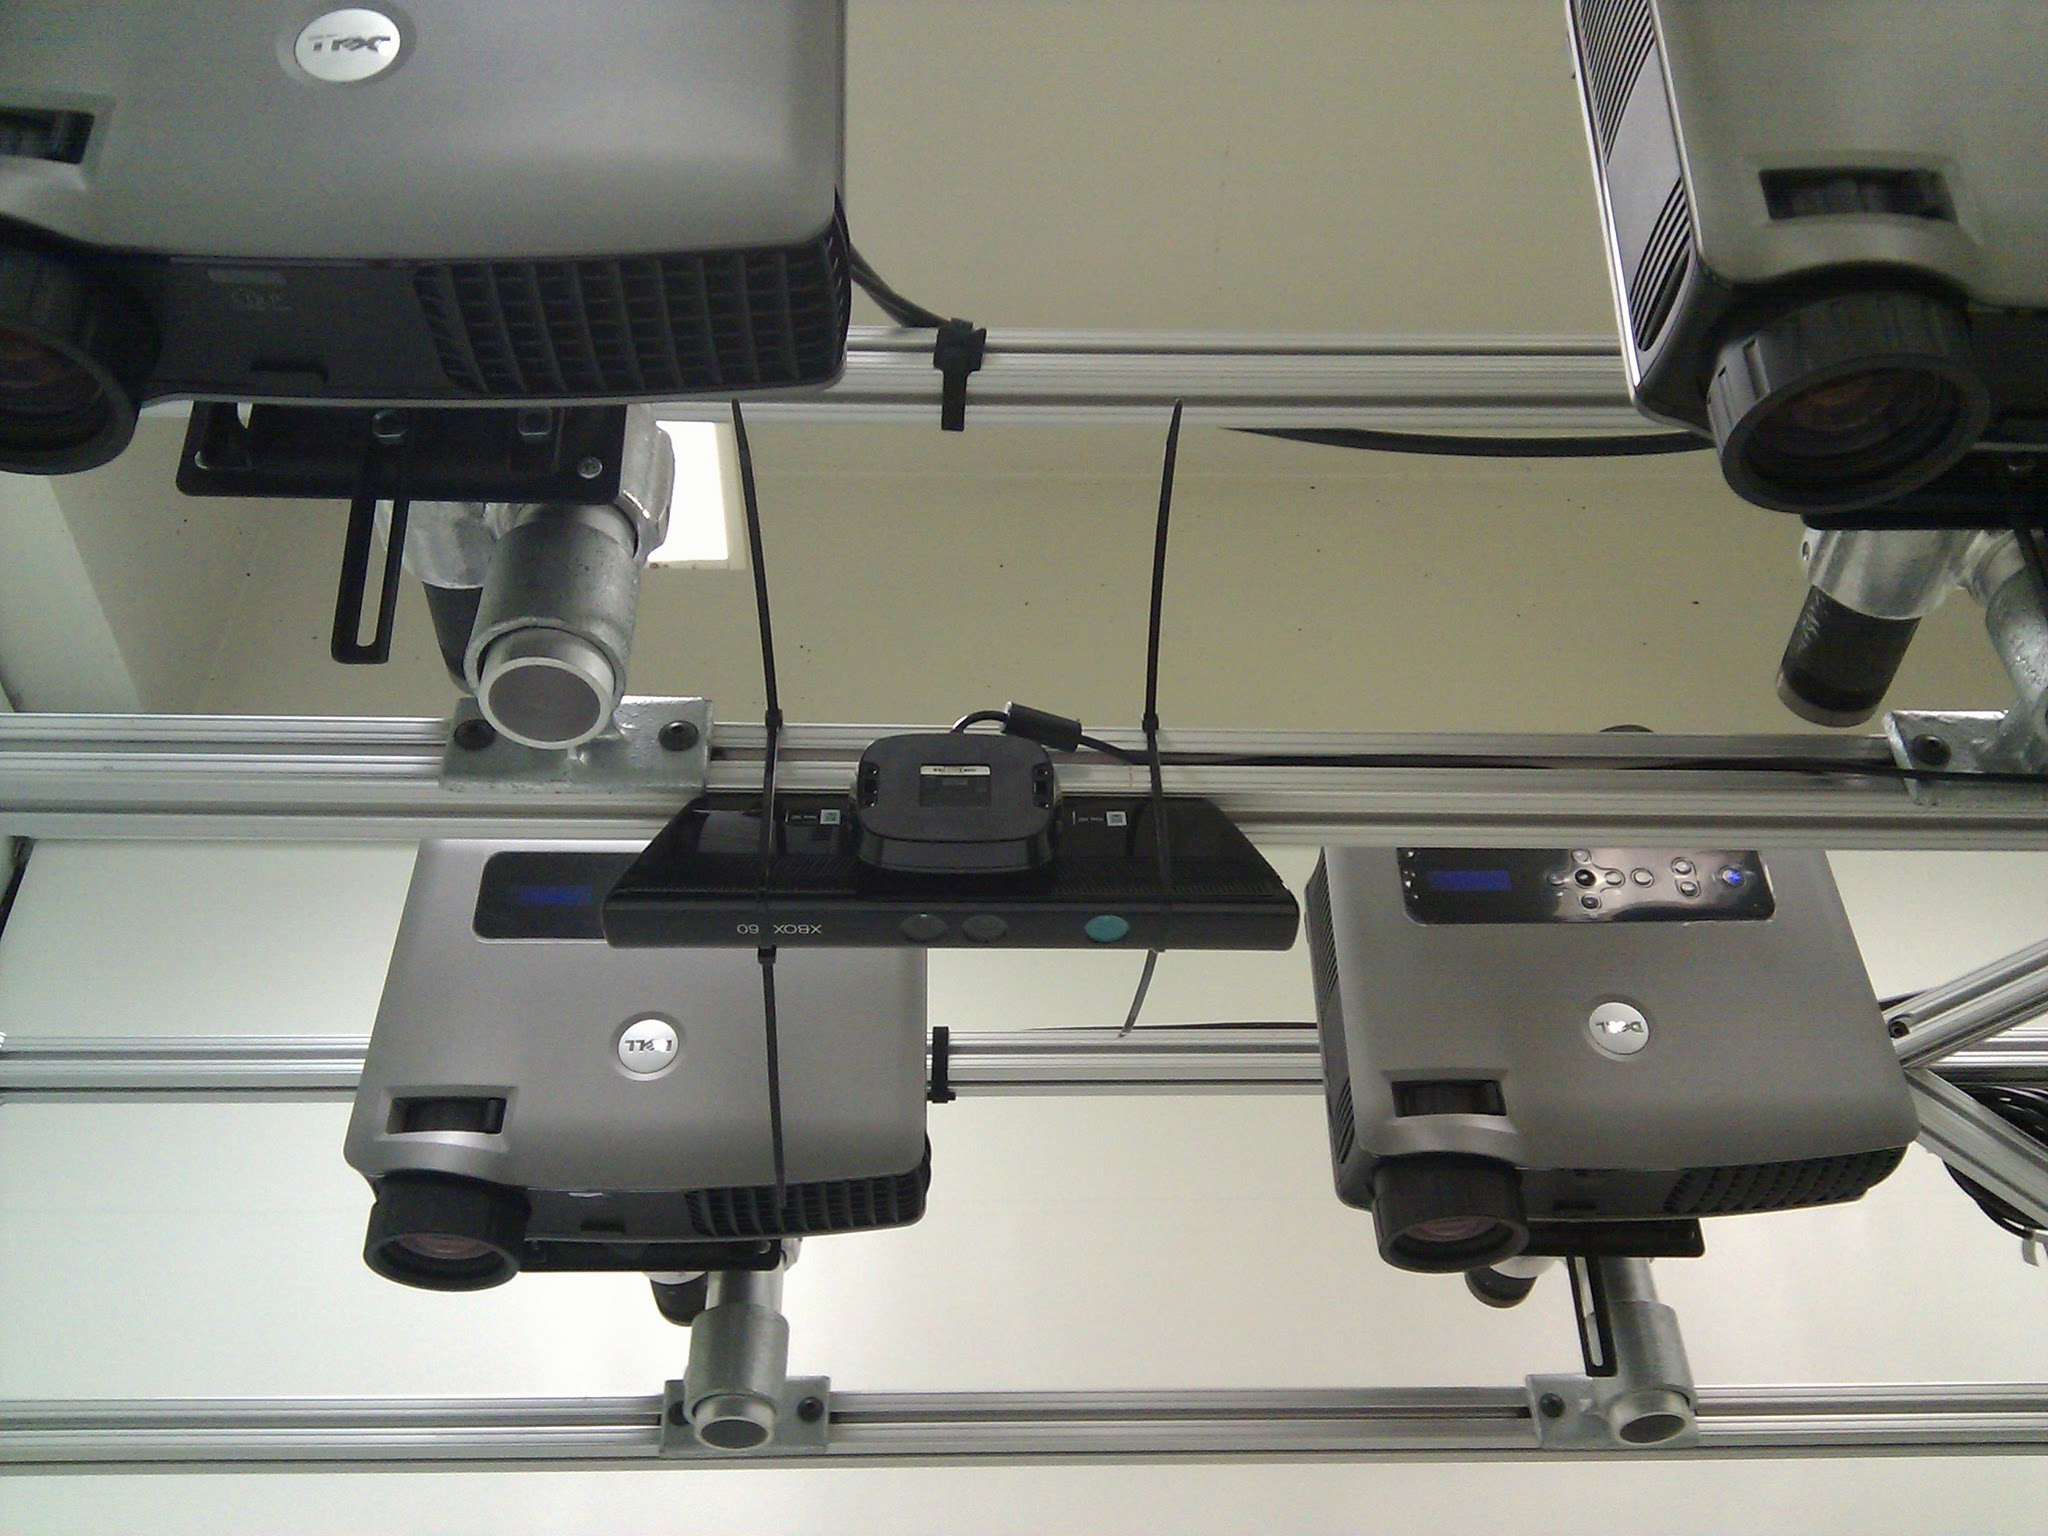
\includegraphics[width=0.4\textwidth]{figures/setup_close.png}
  }
  \caption{System setup.} \label{fig:setup}
\end{figure}

One Kinect motion sensor by Microsoft is placed above the center of the tabletop
at the same level of the projectors. Figure~\ref{fig:setup} shows the setup. The
Kinect sensor has a RGB camera, a depth sensor and a multi-array microphone.
We use the depth sensor to capture hand motion data because it is
less sensitive to the lighting condition. This is particularly useful for our
projection system. The Dell 5100MP projector uses a spinning color wheel to
modulate the image. This produces a visible artifact on the screen, referred to 
as the ``rainbow effect'', with colors separating out in distinct red, green, 
and blue. At any given instant in time, the image on the screen is either red, or green, or blue,
and the technology relies upon people's eyes not being able to detect the rapid 
changes from one to the other. However, when seen through a RGB camera, the
effect is very obvious, and this can greatly affect hand segmentation if we were to use 
the RGB images. 

The Kinect sensor outputs video at a frame rate of 30Hz. The depth sensing video
stream has a resolution of $640\times 480$ pixels with 11-bit depth value. The
depth value increases as the distance of the object from the sensor increases.
The tabletop surface is about 1.2m away from the Kinect
sensor which allows us to have a relatively good depth resolution. We use the
open source OpenNI framework \footnote{https://github.com/OpenNI/OpenNI} and its
Kinect driver \footnote{https://github.com/avin2/SensorKinect} to get both the depth and RGB data streams.

\subsection{Kinect Calibration}
In order to develop an interactive interface, we need to map the point in the
depth image to the point on the display. We do this by projecting a
checkerboard image on the tabletop display, and placing some wooden blocks at
the corners of the checkerboard image to create the depth differences so that 
the depth sensor can capture these corners (see Figure~\ref{fig:calibration}).
We manually labeled 16 pairs of corresponding points on the display and the depth image. Then we
apply undistortion to the depth image and planar homography to find the mapping.

\begin{figure}[h]
  \centering
  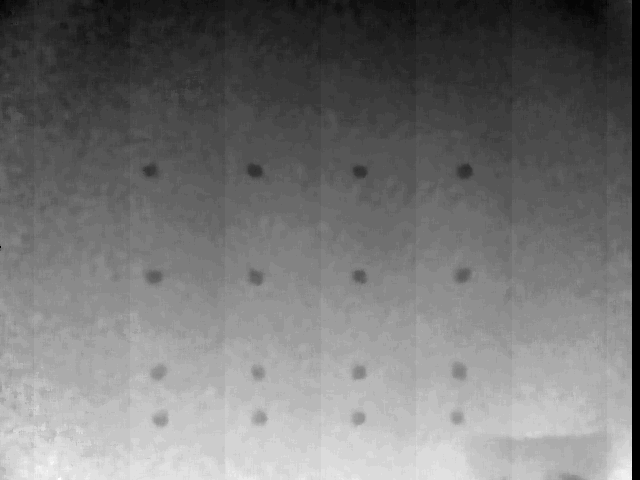
\includegraphics[width=0.5\textwidth]{figures/calibration.png} 
  \caption{Kinect calibration. The darker squares are the wooden blocks. The
  intensity of the gray level image is inversely proportional to the distance
  from the Kinect sensor.}
  \label{fig:calibration}
\end{figure}

Planar homography is a projective mapping from one plane to another. In our
case, we are mapping points on the plane of the depth image to the points
on the plane of the display. To evaluate the result of the calibration, we
obtain a new set of manually labeled corresponding points on the display and the
depth image. We then transform the coordinates of the points on the depth image
to the coordinates on the display using the calibration result, and find the
Euclean distance (error) between the transformed coordinates and the labeled
coordinates of the points on the display. The average errors in the x-axis and
y-axis are 4.3px and 8.9px respectively, which are 0.21cm, and 0.4cm in physical distance of the
projected display. The average width of the index fingertip is about 1.4cm, so
the error is less than 30\% of the width of the fingertip. 

\subsection{Hand Tracking}
The hand tracking process consists of feature detection and parameter estimation. The hand tracking
pipeline consists the following steps:

\begin{enumerate}
  \item Background subtraction
  \item Forelimb and hand segmentation
  \item Fingertips tracking
\end{enumerate}

The following subsections explain in details about these steps. Many of the
computer vision methods we use are based on the OpenCV
\footnote{http://opencv.willowgarage.com/wiki/} library and its Java interface 
JavaCV \footnote{http://code.google.com/p/javacv/}.

\subsubsection{Background Subtraction}
While the background - i.e., the tabletop - is relatively static, there is
still noise from the depth sensor. We use the averaging background method, which
learns the average and average difference of each pixel in the depth image as
the model of the background. The average values are based on the initial 30
frames with no hands in the scene. For the subsequent frames, any value that is 
6 times the average frame-to-frame absolute difference below the average tabletop depth value for that pixel is considered 
foreground because it is closer to the sensor above.

To clean up the background subtracted depth image, we use 1 iteration of
morphological opening to clear out small pixel noise. Morphological opening is a
combination of erosion and dilation. Both erosion and dilation are morphological
transformations. The kernel of erosion is a \textit{local minimum} operator,
while that of dilation is a \textit{local maximum} operator.

\begin{figure}[h]
  \centering
  \subfigure[Without using morphological opening.] {
	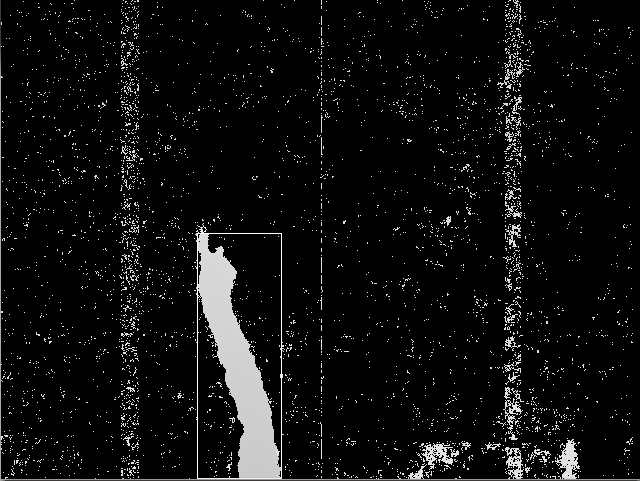
\includegraphics[width=0.4\textwidth]{figures/background_subtraction.png} 
  }
  \subfigure[Using morphological opening to clear out small pixel noise.] {
  	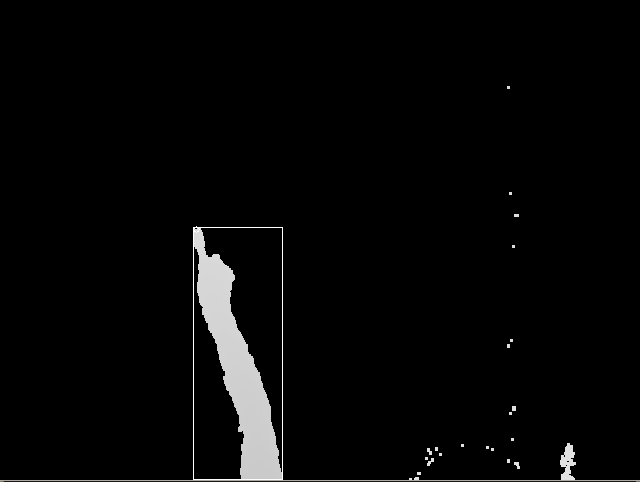
\includegraphics[width=0.4\textwidth]{figures/morphology.png}
  }
  \caption{Background subtraction.} \label{fig:setup}
\end{figure}


\subsubsection{Forelimb and Hand Segmentation}
With the cleaned up background subtracted depth image, we find connected
components by finding all contours that are not too small. These components are
considered to be the forelimbs and are approximated with convex hulls and 
bounding boxes. The hand region is at either end of the bounding box depending
on the position of the arm relative to the table.

\subsubsection{Fingertips Tracking}
We base our estimation of the hand model on geometric properties of the
hand. We compute the convexity defects from the convex hull of the forelimb
(Figure \ref{fig:convexity_defects}). From this we can observe that for an
extended finger, it has one convexity defect on each side and the two adjacent sides of the defects form an
acute angle. We iterate through the adjacent convexity defects, and mark the
intersection of those sides that form an angle smaller than a threshold
value as the potential fingertip. We further refine the fingertip position by
searching in the general direction of the finger and finding a sharp change in
the gradient of the depth value.

\begin{figure}[h]
  \centering
  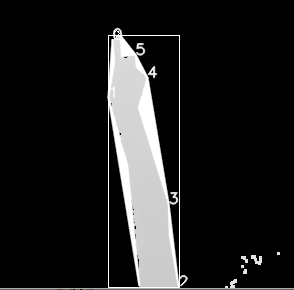
\includegraphics[width=0.4\textwidth]{figures/convexity_defects2.png} 
  \caption{The white triangles are the convexity defects.}
  \label{fig:convexity_defects}
\end{figure}

\subsubsection{Kalman Filter}
We use a Kalman filter to further improve tracking accuracy. The dynamic state
of the fingertip can be summarized by a $4$-dimensional vector, $x_k$, including
two position variables, $x$ and $y$, and two velocities, $v_x$ and $v_y$. The
measurement is a $2$-dimensional vector, $z_k$, of the measured $x$ and $y$ coordinates of the fingertip.

Assuming no external control, the a priori estimate $x_k^-$ of the state is
given by:
\begin{align*}
x_k^- = Fx_{k - 1} + w_k
\end{align*}
$F$ is the $4$-by-$4$ \textit{transfer matrix} characterizing the
dynamics of the system with the following values:

\begin{align*}
x_k = \begin{bmatrix}
	x   \\
	y   \\
	v_x \\
	v_y \end{bmatrix}_k, \quad
F = \begin{bmatrix}
	1 & 0 & 1 & 0 \\
	0 & 1 & 0 & 1 \\
	0 & 0 & 1 & 0 \\
	0 & 0 & 0 & 1 \end{bmatrix}
\end{align*}
assuming constant velocities, and that time is measured in frames.
$w_k$ is the \textit{process noise} associated with random events or forces
that directly affect the actual state of the system. We assume that the 
components of $w_k$ have Gaussian distribution $N(0, Q_k)$ for some $4$-by-$4$ 
covariance matrix $Q_k$. We set the matrix $Q$ with the following values:
\begin{align*}
Q = \begin{bmatrix}
	1 & 0 & 0 & 0 \\
	0 & 1 & 0 & 0 \\
	0 & 0 & 10 & 0 \\
	0 & 0 & 0 & 10 
	\end{bmatrix}
\end{align*}
The larger variance values indicate the greater uncertainty in the velocities as
they may not be constant.

\subsubsection{Evaluation}
We evaluate the accuracy of our fingertip tracking method by comparing the
detected fingertip position with the manually labeled position in a sequence of
video frames. In this first evaluation, only one extended finger is used. Our
method finds all the labeled fingertips and the average error (Euclean distance)
is 5.3px which is about 10mm. In their finger click evaluation, Harrison et al.
reports that their system has an average of 11.7mm offset from the targets. 

Here we want to emphasize that the focus of the thesis is gesture recognition
and finding a hand model that is suitable for gestural input. As a result, we
are not pushing the accuracy of fingertip and click detections to as high as
possible. We also envision that better touch screen hardware will be developed
in the near future with larger size and higher resolution, and hence, touch
detection accuracy can be very high. Our hand model and gesture analysis
framework should be general enough such that it can be easily adapted to
different sensor inputs.

\section{Hand Tracking for Seated Interaction with Vertical Display}
\subsection{Gesture Salience Detection}
Similar to Marcos-Ramiro et al.~\cite{marcos2013}, we define gesture
\textit{salience} as a function of both the closeness of the motion to the
observer (e.g., the camera) and the magnitude of the motion.
There are 4 steps in our method (Figure~\ref{fig:gesture-salience}).

\begin{figure*}[tb]
\centering
\hspace{-0.6em}%
\subfigure[]{
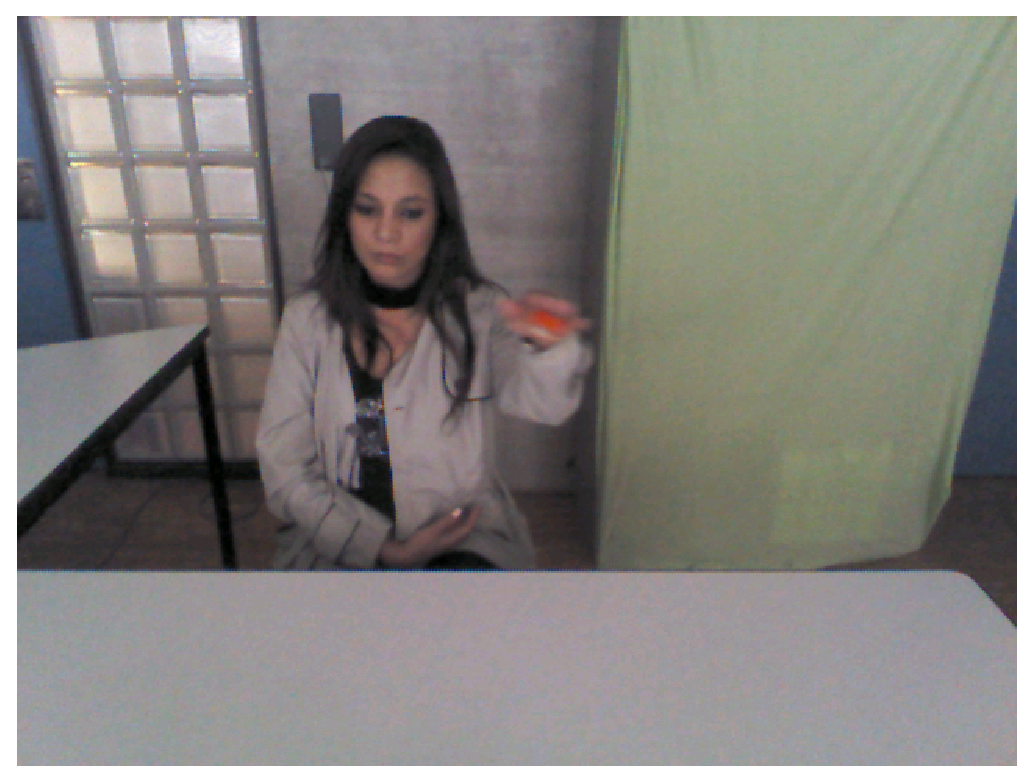
\includegraphics[width=0.19\linewidth]{figures/color.eps}\hspace{-0.6em}%
\label{fig:color}
}
\subfigure[]{
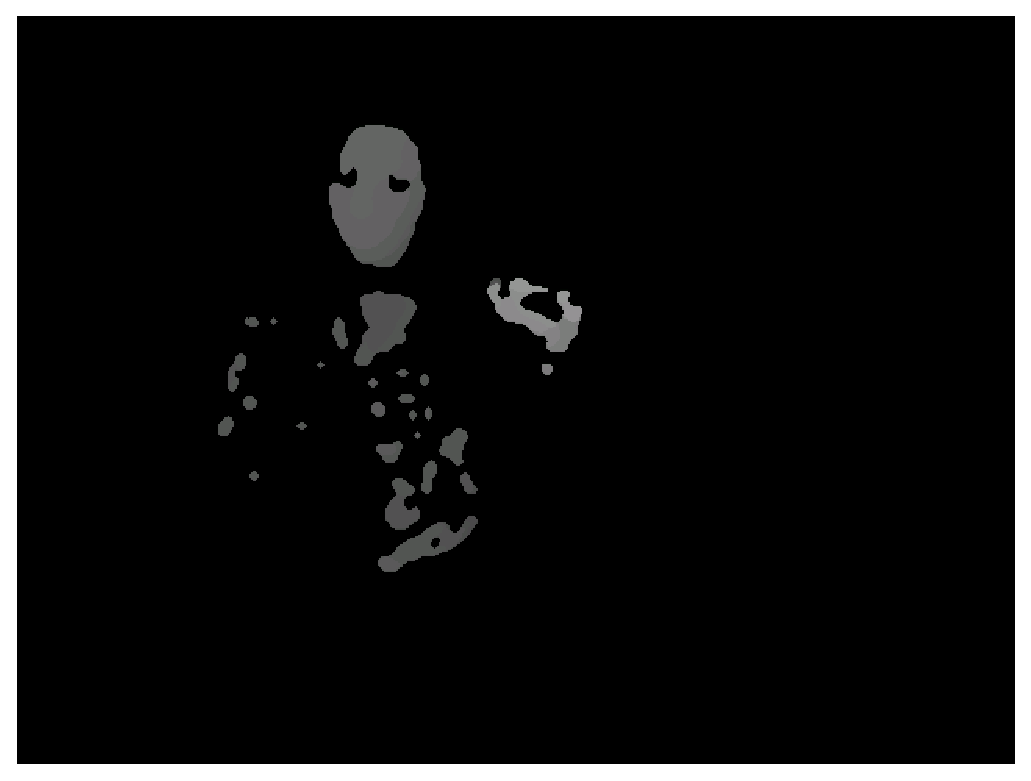
\includegraphics[width=0.19\linewidth]{figures/depth.eps}\hspace{-0.6em}
\label{fig:skin-mask}
}
\subfigure[]{
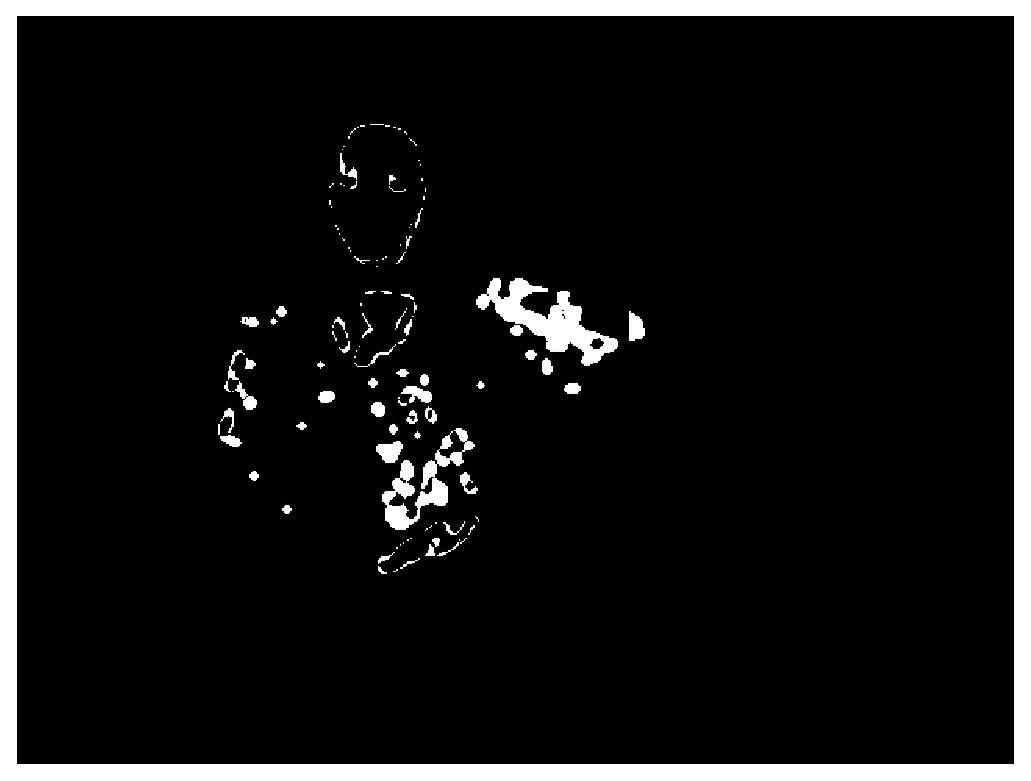
\includegraphics[width=0.19\linewidth]{figures/motion-mask1.eps}\hspace{-0.6em}
\label{fig:motion-mask}
}
\subfigure[]{
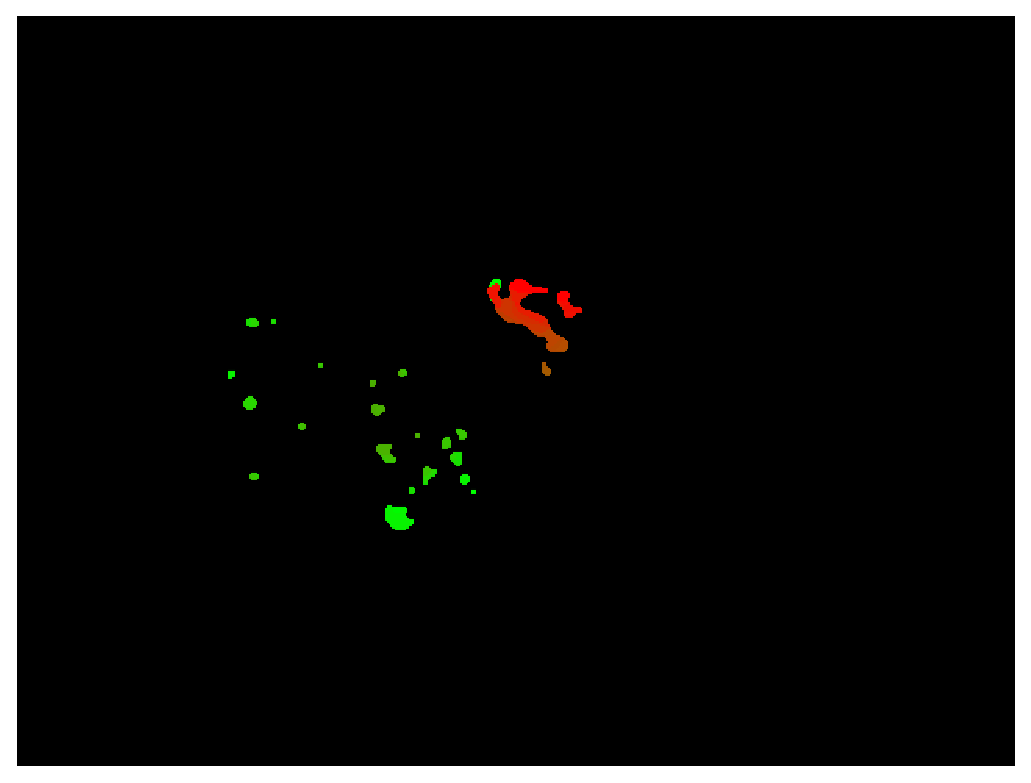
\includegraphics[width=0.19\linewidth]{figures/salient-map.eps}\hspace{-0.6em}
\label{fig:salience}
}
\subfigure[]{
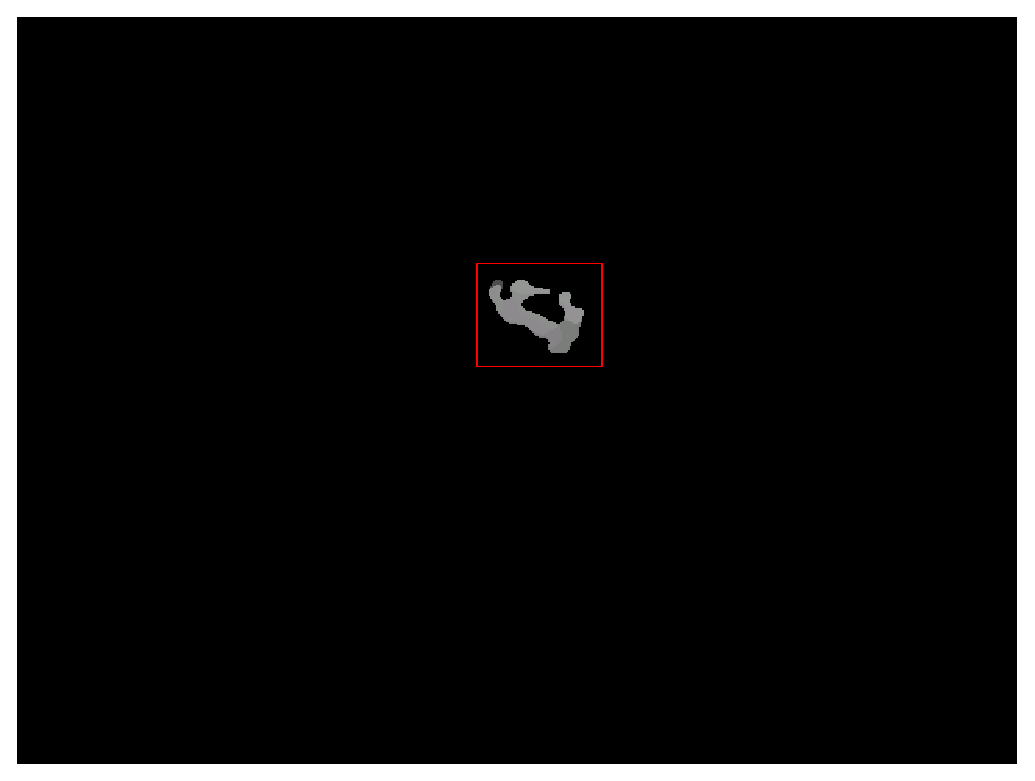
\includegraphics[width=0.19\linewidth]{figures/bounding-box.eps}
\label{fig:camshift}
}
\caption{Gesture salience detection steps: \subref{fig:color} RGB image under low lighting condition;
\subref{fig:skin-mask} depth map $D_t$ filtered by skin and user mask, $M_t^{S\wedge U}$. False detection of skin is due to
the similar colors between clothes and skin; \subref{fig:motion-mask} motion mask,  $M_{t\vee t-1}^M$, indicating moved pixels for time $t$ and $t-1$;
\subref{fig:salience} salience map with red color indicating high probability of the salience;
\subref{fig:camshift} final gesture salience bounding box, $B_t$. (Best viewed in
color. Based on data from ChAirGest corpus~\cite{Ruffieux2013}.)}
\label{fig:gesture-salience}
\end{figure*}

\subsubsection{Skin Segmentation}
We use an off-the-shelf simple skin color detection method to compute a binary skin mask at
time $t$, $M_t^S$, based on the RGB image. We also find the user mask, $M_t^U$ obtained from the Kinect SDK based on the depth image.
We align the two to find their intersection $M_t^{S\wedge U}$, which indicates the user's skin region.

\subsubsection{Motion Detection}
The depth data is first clipped to a maximum value $\text{depth}_\text{max}$ of
2m and then scaled to a value between 0 and 255 (1 byte):

\begin{align*}
\text{scaled} = (\text{depth}_\text{max} -
\text{depth}_\text{clipped}) \times 255 / \text{depth}_\text{max}
\end{align*}

The scaled value is inversely proportional to the depth value.
We compute the motion mask for the current depth frame based on 3 frames. We first filter each
depth frame by the user and skin mask $M_t^{S\wedge U}$, and then
smooth it through a median filter to obtain $D_t$ (Figure~\ref{fig:skin-mask}).
Equation~(\ref{eq:motion-mask}) computes the binary mask, $M_{t\vee t-1}^M$,
indicating pixels whose depth values have changed from time $t-1$ to $t$ (Figure~\ref{fig:motion-mask}).
$D_{t\vee t-1}$ is the absolute difference between $D_t$ and $D_{t-1}$, and $T$ is the threshold operator that filters out small changes in depth value
(with a threshold of 15mm).
To obtain the motion mask, $M_{t}^M$ for time $t$ only, we use $M_{t-1\vee t-2}^M$, the motion mask for $t-1$ and $t-2$ as well (see Equation~(\ref{eq:motion-mask-t}),
 AND and XOR are indicated by $\wedge$ and $\oplus$).
\begin{align}
M_{t\vee t-1}^M &= T(D_{t\vee t-1}) \label{eq:motion-mask} \\
M_{t}^M &= M_{t\vee t-1}^M \oplus (M_{t\vee t-1}^M \wedge M_{t-1\vee t-2}^M) \label{eq:motion-mask-t}
\end{align}

\subsubsection{Salience Map}
We compute histograms of depth values in both $D_t$ and $D_{t\vee t-1}$ and then apply histogram normalization to obtain cumulative distributions $H_t$ and $H_{t\vee t-1}$.
$H_t$ represents the probability of salience given a depth value, while $H_{t\vee t-1}$ represents the probability of salience given
a depth difference value. The lower the depth value or the higher the depth difference value, the higher the salience probability. We use
histogram equalization to reduce the effect of outliers, so that a single large depth value will not suppress the salience probabilities of other depth values.
The salience map (Figure~\ref{fig:salience}) can then be computed for each pixel $(x, y)$:
\begin{align*}
S_t(x, y) = H_t(D_t(x, y)) \times H_{t\vee t-1}(D_{t\vee t-1}(x, y)) \times M_t^M
\end{align*}
The multiplication of the binary motion mask $M_t^M$ allows us to consider only the motion due to the user at $t$.

\subsubsection{Salience Location}
The final step of locating the most salient region in a frame is finding the
contour, $C_t$, from the salience map $S_t$ that has a perimeter greater than
the smallest possible hand perimeter and with the highest average salience for all the pixels inside the contour.

When motion is slow, the motion mask usually indicates the edge of the moving
object. As a result, the center of $C_t$ may not be the center of the moving
object (in our case, the user's hand). Hence, we use 2 iterations of Camshift~\cite{Bradski98} on
the depth image $D_t$ with a starting search location at the center of $C_t$ to refine
the final bounding box, $B_t$, of gesture salience (Figure~\ref{fig:camshift}).

Figure~\ref{fig:compare-skeleton} shows examples of our hand tracking result (red regions).
It is more reliable than the hand joint locations from the Kinect SDK. In the
Experimental Evaluation section (Section~\ref{sec:eval}), we show that using our
salience detection method to extract hand position features gives 3.7\%
absolute increase in gesture recognition F1 score compared to using the hand
joint position from the Kinect SDK.

\begin{figure*}
\centering
\subfigure[]{
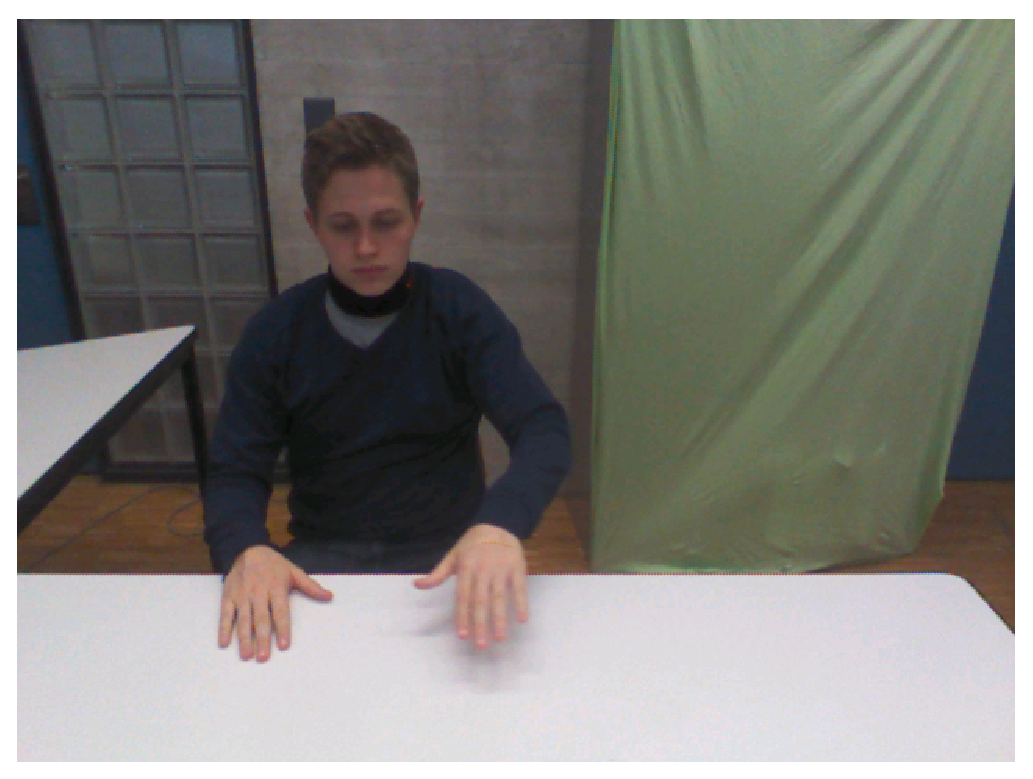
\includegraphics[width=0.23\linewidth]{figures/rotate-color.eps} \hspace{-0.6em}
}
\subfigure[]{
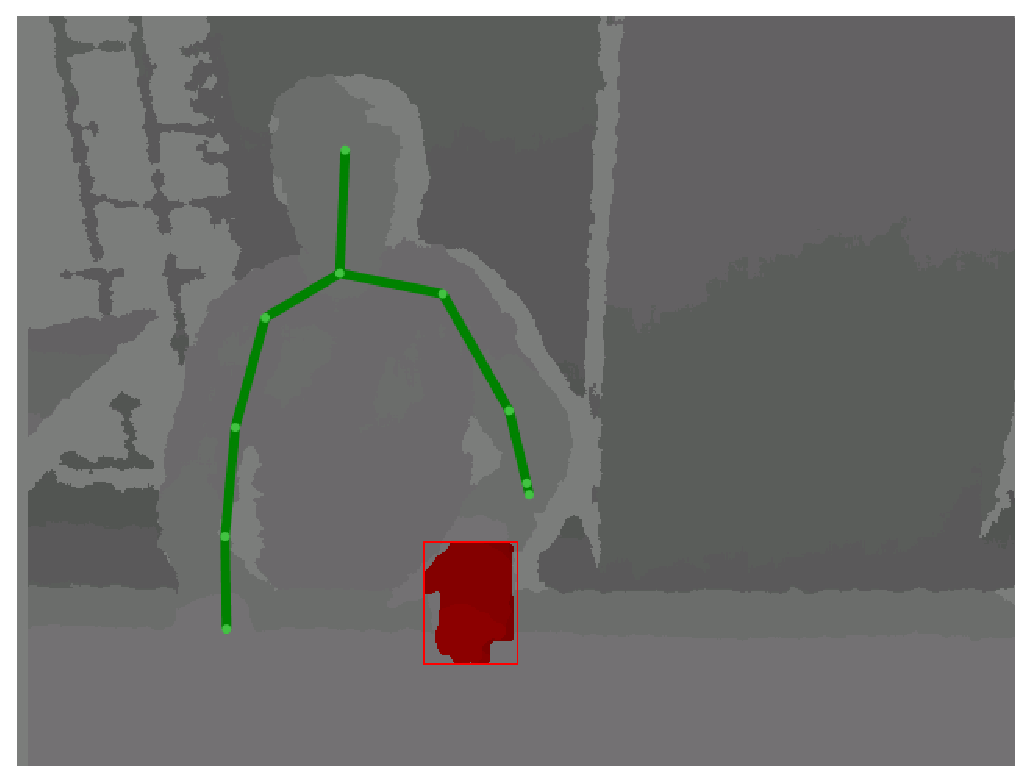
\includegraphics[width=0.23\linewidth]{figures/rotate-depth.eps} \hspace{-0.6em}
}
\subfigure[]{
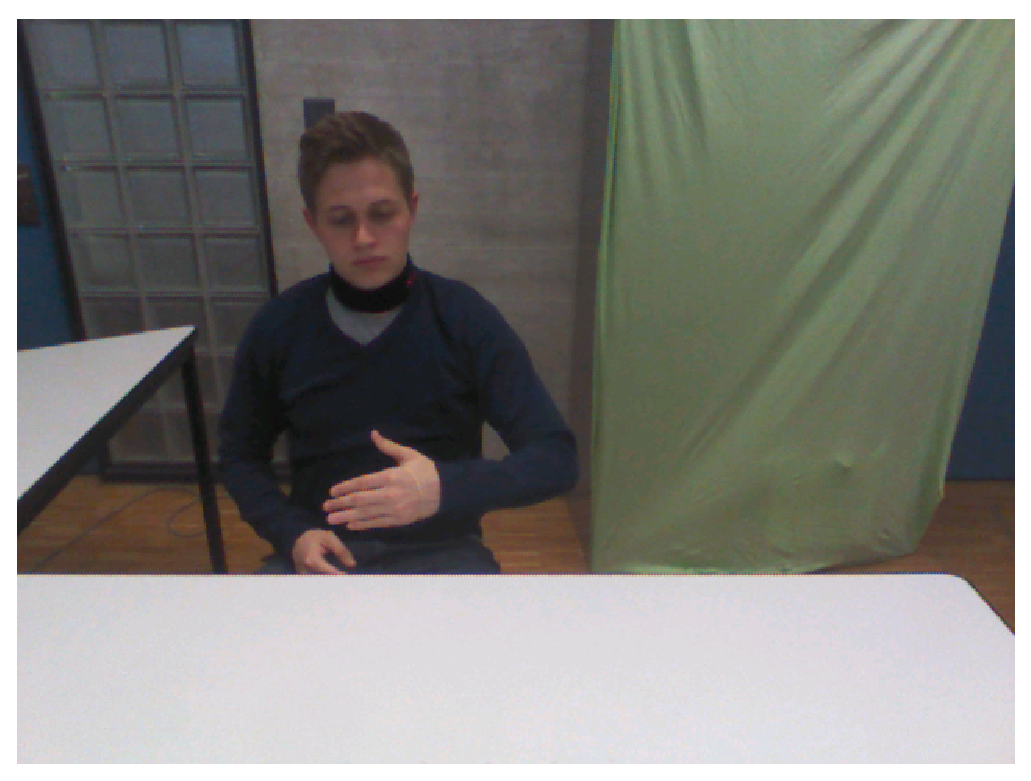
\includegraphics[width=0.23\linewidth]{figures/near-body-color.eps}
\hspace{-0.6em} }
\subfigure[]{
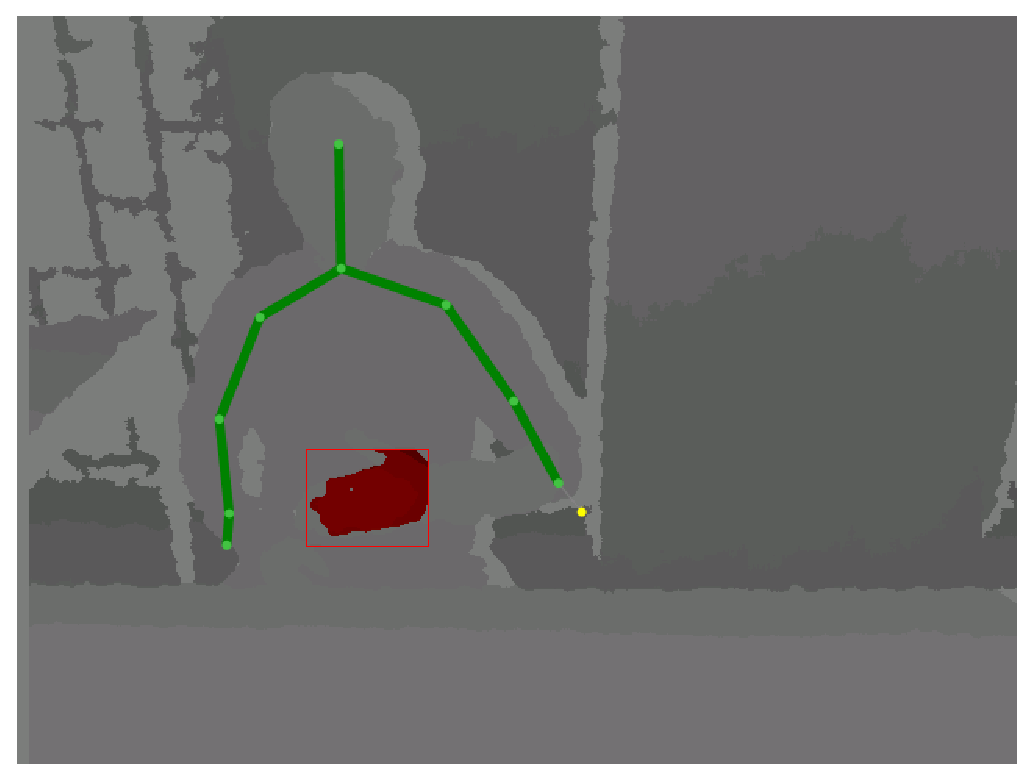
\includegraphics[width=0.23\linewidth]{figures/near-body-depth.eps}
\hspace{-0.6em} }
\caption{Comparison of hand tracking results. Our method (red region) gives more
reliable result on hand tracking compared to the off-the-shelf Kinect software
(green line). (Best viewed in color. Based on data from ChAirGest
corpus~\cite{Ruffieux2013}.)}
\label{fig:compare-skeleton}
\end{figure*}


\section{Hand Tracking and Feature Extraction}
As one category of gestures is characterized by distinct hand poses,
we need to track the full hand, rather than just treating the hand as one point. We
also need to derive a feature vector that represents the hand shape as well.

We base our hand tracking on information from the skeleton tracking of the
Kinect SDK, which is relatively robust for standing articulated body poses. At
each time frame, we use the hand joint position reported from the SDK as an
initial rough estimate of the bounding box of the hand in the depth frame.
We align the RGB and the depth frames, use skin detection to filter out
non-skin pixels in the bounding box, and then refine the bounding box using 4
interactions of CAMSHIFT \cite{bradski98}. We normalize the bounding box to a $32\times 32$ px depth
mapped image. We compute HOGs
feature from the normalized hand image (cell size =
4, number of orientation bins = 9) (see Fig.~\ref{fig:tracking}).
Since the depth data is less affected by change in illumination, we use only one
fold of normalization in the HOG feature to speed up processing.
This gives us a HOG feature of length 441 ($(32/4 - 1)\times (32/4 - 1)\times 9$). The HOG
feature has been used as a hand pose descriptor in previous work \cite{song12}
where it is often used as the input to a classifier such (e.g., Support Vector
Machine (SVM)). Our system uses principal component analysis (PCA)
to reduce the HOD dimensionality from 441 to 14, then uses it directly as part
of the input feature vector to the hidden Markov model (HMM) based recognition framework.

\begin{figure}[!t]
\centering
\includegraphics[width=0.8\columnwidth]{fig/hand_tracking.ps}
\caption{Hand tracking and hand pose feature extraction.}
\label{fig:tracking}
\end{figure}